\chapter{مقدمه}

آژانس بین‌المللی انرژی، بهره‌وری انرژی در ساختمان‌ها را به عنوان یکی از پنج اقدام برای تضمین کربن‌زدایی طولانی‌ مدت بخش انرژی شناسایی کرده است\cite{DEB2017902}
در کنار مزایای زیست محیطی، بهره‌وری انرژی ساختمان دارای مزایای اقتصادی گسترده ای نیز می‌باشد.
 ساختمان‌هایی با سیستم‌های انرژی کارآمد و استراتژی‌های مدیریتی هزینه‌های عملیاتی بسیار کمتری دارند. اکنون بسیاری از کشورها اجرای قوانین و مقررات انرژی را
 برای انواع ساختمان‌ها تسریع کرده‌اند. این مقررات الزامات اساسی برای دستیابی به یک طراحی کارآمد انرژی برای ساختمان‌های 
 جدید با هدف کاهش مصرف انرژی نهایی و انتشار \lr{CO2} مرتبط را ترسیم می‌کند. 
 علاوه بر این، بسیاری از نرم افزارهای کامپیوتری نیز برای طراحی بهینه انرژی ساختمان‌های جدید توسعه یافته 
 و به طور گسترده پیاده‌سازی شده‌اند. در مورد تکنیک‌های موجود تجزیه و تحلیل انرژی ساختمان
  به کمک کامپیوتر و ابزارهای نرم‌افزاری در \cite{ALHOMOUD2001421, CRAWLEY2008661} اطلاعات دقیقی موجود هستند. این مقررات و ابزارهای کامپیوتری مربوط
   به ساختمان‌های جدید است و در واقع بسیار موثر هستند. با این حال، هنگامی که ساختمان در حال فعالیت است، عوامل زیادی بر رفتار
   انرژی یک ساختمان حاکم هستند، مانند شرایط آب و هوایی، برنامه حضور ساکنین ساختمان، خواص حرارتی مصالح ساختمانی، فعل و انفعالات پیچیده 
  سیستم‌های انرژی مانند گرمایش و تهویه‌هوا و روشنایی و غیره. به دلیل این فعل و انفعالات پیچیده،
   محاسبه دقیق مصرف انرژی از طریق مدل شبیه‌سازی کامپیوتری بسیار دشوار است. به این دلایل، تکنیک‌های داده‌محور برای تجزیه و تحلیل مصرف انرژی ساختمان‌های
   موجود بسیار حیاتی است. این تکنیک‌ها بر داده‌های ثبت‌شده گذشته تکیه دارند و
   تلاش می‌کنند مصرف انرژی را بر اساس الگوهای مصرف انرژی قبلی مدل‌سازی کنند. سایر عوامل مؤثر بر مصرف انرژی را می توان برای بهبود
    دقت چنین مدل‌های سری زمانی استفاده کرد. این تکنیک‌ها که از داده‌های گذشته استفاده می‌کنند،
    اغلب تحت «یادگیری ماشین» قرار می‌گیرند و در دو دهه اخیر به طور فعال در مطالعات پیش‌بینی انرژی ساختمان به کار رفته‌اند

\section[اهمیت بهینه سازی عملکرد ساختمان‌ها]{اهمیت بهینه سازی عملکرد ساختمان‌ها\cite{DEB2017902}}

برای دستیابی به سطح بهینه عملکرد انرژی در ساختمان‌ها، نصب سیستم‌های انرژی کارآمد باید با استراتژی‌های عملیاتی و مدیریتی مناسب دنبال شود. 
این امر مستلزم نظارت و مدیریت مداوم داده‌های انرژی سری زمانی همراه با سایر عوامل موثر بر عملکرد انرژی ساختمان ها است. 
در رابطه با نظارت مستمر و مدیریت مصرف انرژی در ساختمان های موجود، پیش‌بینی نقش بسزایی دارد. می‌تواند مجموعه‌ای از شرایط مرزی و اهداف را برای مدیران و 
مالکان تأسیسات ساختمانی فراهم کند که مصرف انرژی ساختمان به طور ایده‌آل باید در آن قرار گیرد (هدف‌های روزانه، هفتگی، ماهانه و سالانه). 
همانطور که مدل پیش‌بینی سری‌های زمانی از الگوهای مصرف انرژی قبلی یاد می‌گیرد، افزایش تدریجی مقادیر مصرف انرژی پیش‌بینی‌شده
 در یک دوره زمانی ممکن است مدیران تأسیسات را در مورد جنبه‌های تعمیر و نگهداری ساختمان و سیستم‌های انرژی آگاه کند. 
علاوه بر رویکرد پیش‌بینی سری‌های زمانی، سایر رویکردهای سری غیرزمانی را می‌توان برای اهداف بهینه‌سازی ساختمان اتخاذ کرد
 و همچنین می‌توان آنها را با سایر مدل‌های شبیه‌سازی کامپیوتری برای استخراج اشغال و
  سایر عوامل عملیاتی ترکیب کرد.
  \\
   یانگ\LTRfootnote{\lr{Yang}} و همکاران در بهینه سازی انرژی مبتنی بر شبیه سازی برای یک ساختمان آزمایشی در 
  اسپانیا، یک چارچوب بهینه‌سازی الگوریتم ژنتیک موازی
  مبتنی بر وب \LTRfootnote{\lr{GA}} که از منابع محاسباتی توزیع‌شده استفاده می‌کند تا زمان محاسبه
   را کاهش دهد استفاده کردند.پتری \LTRfootnote{\lr{Petri}} و همکاران یک سیستم بهینه‌سازی مبتنی بر مدولار ارائه کردند
    که شبیه‌سازی انرژی و بهینه‌سازی را با استفاده از شبکه عصبی مصنوعی ترکیب می‌کند.
    این برنامه کاهش قابل توجه انرژی (کیلووات ساعت) را در یک سناریوی واقعی نشان داد.
    با این حال، این امر مستلزم تجهیز ساختمان به حسگرها و عملگرها برای نظارت، کنترل
    و بهینه سازی بود. این ممکن است در مورد اکثر زیرساخت های ساختمان موجود نباشد.
    چنین چالش هایی مورد بحث قرار می گیرند. با این حال، همچنین خاطرنشان می شود
    که پتانسیل صرفه جویی انرژی مرتبط در ساختمان ها به راه اندازی، ردیابی عملکرد
    و استراتژی های کنترل پیشرفته مربوط می شوند. این امر به عوامل بسیاری از جمله منابع مالی،
    حمایت از سیاست، آگاهی سبز، مواد سبز و فناوری و غیره وابسته است.
    \\
    زونگ\LTRfootnote{\lr{Zong}} و همکاران در مورد چالش های اجرای یک مدل اقتصادی 
    استراتژی کنترل پیش بینی \LTRfootnote{\lr{EMPC}} برای ساختمان های هوشمند بحث کردند. مشاهده شد که هنوز چالش‌هایی
     در کاربرد کنترل پیش‌بینی مدل از جمله سازش بین ساده‌سازی و پیچیدگی مدل‌سازی 
    دینامیکی حرارتی ساختمان و تعادل بین سیستم‌های چند انرژی وجود دارد.
     هو و همکاران با درک چالش‌ها در ادغام داده‌های عملکرد ساختمان
     با سایر داده‌های مربوط به ساختمان. روش جدیدی را برای پیوند
     دادن داده‌های قطع شده سنتی برای ساخت منابع داده ارائه کرد تا 
    ارزیابی عملکرد ساختمان را به صورت عمیق و روشن‌تر فراهم کند. 
پیش‌بینی سری‌های زمانی برای بهینه‌سازی عملکرد ساختمان ضروری است. هر تکنیک بهینه‌سازی به
 اطلاعاتی در مورد سناریوهای آینده یا یافتن بهترین راه‌حل‌ها در برابر یک معیار
  آزمایشی نیاز دارد. تکنیک های یادگیری ماشین در این زمینه مفید هستند و اغلب در حل این دو مشکل استفاده می شوند. 
با این حال، این بررسی بر جنبه‌های پیش‌بینی سری‌های زمانی بهینه‌سازی ساختمان تمرکز دارد تا اینکه به طور کلی به مسئله بهینه‌سازی نگاه کند. ادغام این دو باید در یک بررسی جداگانه مورد بررسی قرار گیرند.



\section[اهداف بررسی]{اهداف بررسی\cite{DEB2017902}}
مطالعات بررسی اخیر در مورد پیش بینی انرژی، گزارش‌های دقیقی از مدل های پیش بینی موجود و طبقه بندی آنها ارائه می دهد.ژائو \LTRfootnote{\lr{Zhao}} و ماگولس\LTRfootnote{\lr{Magoules}} روش های موجود برای پیش بینی مصرف انرژی ساختمان را در پنج دسته بررسی و طبقه بندی کردند. هیپرت\LTRfootnote{\lr{Hippert}} و همکاران مروری بر پیش بینی بار کوتاه مدت ارائه کرد. سوگانتی\LTRfootnote{\lr{Suganthi}} و ساموئل\LTRfootnote{\lr{Samuel}} مروری بر مدل های تقاضای انرژی برای پیش بینی تقاضا ارائه کردند. فومو\LTRfootnote{\lr{Fumo}} مروری بر برآورد انرژی ساختمان ارائه کرد و همچنین نحوه طبقه بندی مدل های برآورد را مورد مطالعه قرار داد. مارتینز-آلوارز\LTRfootnote{\lr{Martinez-Alvarez}} و همکاران یک نظرسنجی در مورد تکنیک های داده‌کاوی برای پیش بینی سری های زمانی الکتریسیته ارائه کرد. این نظرسنجی بر روی ویژگی های مدل‌ها و پیکربندی آنها متمرکز بود. رضا و خسروی مروری بر تکنیک‌های پیش‌بینی بار کوتاه‌مدت بر اساس تکنیک‌های هوش مصنوعی ارائه کردند. مطالعه اخیر توسط مت داوت\LTRfootnote{\lr{Mat Daut}} و همکاران مروری بر تحلیل پیش‌بینی مصرف انرژی الکتریکی ساختمان با استفاده از روش‌های مرسوم و هوش مصنوعی ارائه کرد. 
همه این بررسی‌ها اطلاعات حیاتی در مورد مدل‌های پیش‌بینی انرژی در مقیاس‌های مختلف ارائه می‌کنند و بر عملکرد برتر مدل‌های ترکیبی تأکید می‌کنند. یک مدل پیش‌بینی می‌تواند مبتنی بر داده‌های استاتیکی باشد که معمولا یک متغیر وابسته را با مجموعه‌ای از متغیرهای مستقل منطبق می‌کند، یا می‌تواند از داده‌های سری زمانی منفرد یا موازی استفاده کند. 
\\
این مطالعه بر تکنیک های پیش بینی با استفاده از داده های سری زمانی تاکید دارد. اهمیت تجزیه و تحلیل سری های زمانی به دلیل افزایش آگاهی در جمع آوری و پایش داده ها در زمان واقعی است. مصرف انرژی سری زمانی را نیز می توان با داده های سری زمانی شرایط محیطی داخل ساختمان تنظیم کرد. با استقرار حسگرهای بیشتر در ساختمان‌ها و جمع‌آوری داده‌های سری زمانی بیشتر، یک چارچوب مناسب برای تجزیه و تحلیل و شناسایی قابلیت‌های پیش‌بینی مهم است. هدف این بررسی درک تکنیک‌های پیش‌بینی سری‌های زمانی موجود و ارائه مزایا و چالش‌های آن‌ها است. ارزیابی دقیق مدل ترکیبی نیز به دلیل استفاده فزاینده در ادبیات ارائه شده است. از آنجایی که ترکیبات مدل ترکیبی بسیار زیاد است، اینها در بخش بعدی پس از بررسی انتقادی تکنیک‌های اصلی مانند شبکه ی عصبی مصنوعی\LTRfootnote{\lr{artifical neural network}} و میانگین متحرک خودهمبسته یکپارچه\LTRfootnote{\lr{ARIMA}} مورد بررسی انتقادی قرار می‌گیرند. این مقاله مروری همچنین باید مبنایی برای مقایسه کیفی و کمی برای تمام ۶ تکنیک ذکر شده در اینجا فراهم کند. شایان ذکر است که مدل ترکیبی به عنوان یکی از تکنیک های موجود در بین 6 تکنیک ارائه شده در نظر گرفته شده است. در مدل ترکیبی، در مجموع 29 ترکیب وجود دارد که در این بررسی به آنها پرداخته شده است
\\[3em]
\noindent
اهداف این مقاله مروری عبارتند از:
\begin{itemize}
    \item ارائه بررسی‌ای جمعی و جامع از تکنیک‌های اصلی هوش مصنوعی پیش‌بینی سری‌های ‌ز‌‌مانی با توجه به مصرف انرژی ساختمان
    \item انجام یک تحلیل تطبیقی که شامل هر دو جنبه کیفی و کمی این تکنیک‌ها باشد
    \item تشریح ترکیبات مختلف مدل ترکیبی در حین ارزیابی عملکرد و تازگی آن‌ها
\end{itemize}
\begin{figure}[ht!]
    \begin{center}
        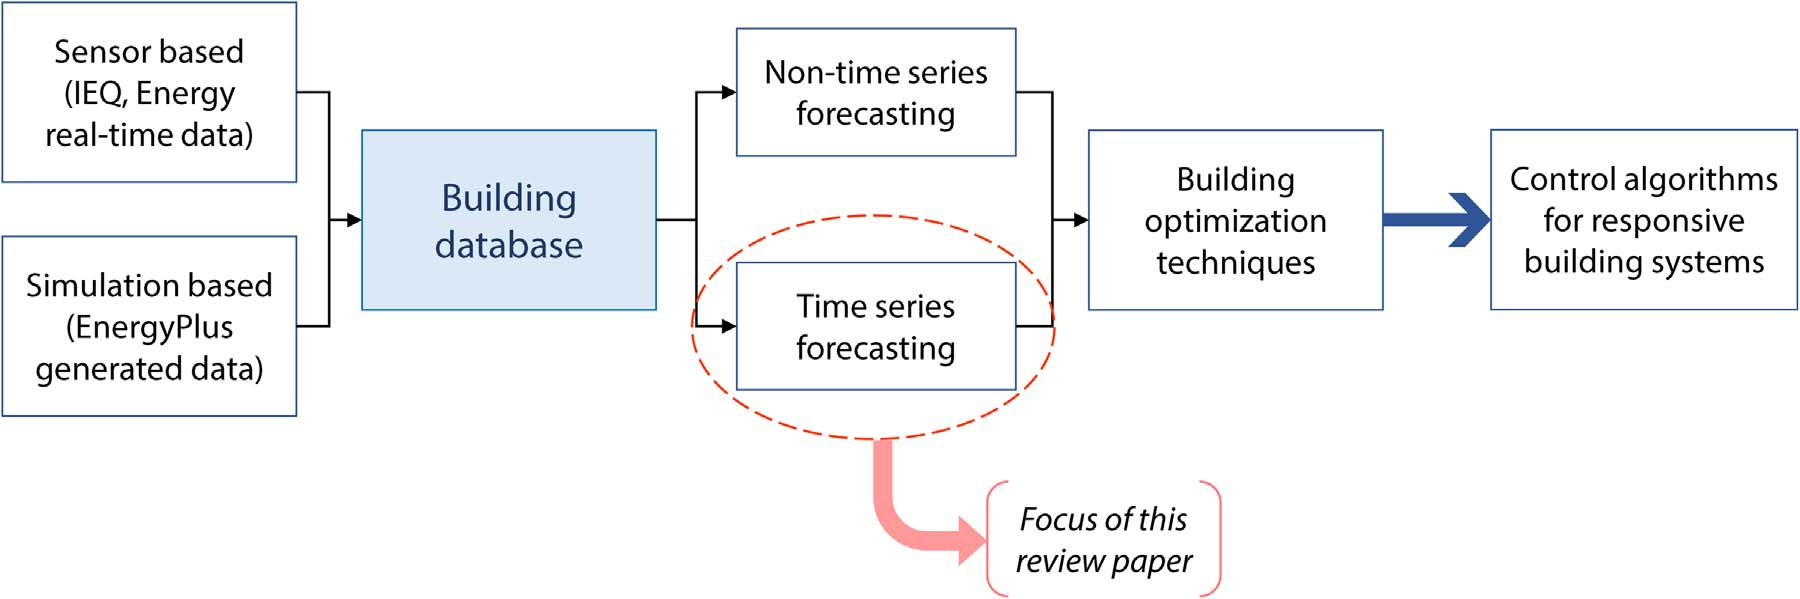
\includegraphics[width=14cm]{images/illustration.jpg}
    \end{center}
    \caption[‌اهمیت پیش‌بینی انرژی ساختمان‌ها برای بهینه سازی ساختمان‌ها]{تمرکز این گزارش نوشتاری در حوزه بهینه‌سازی ساختمان
     \cite{DEB2017902}}
    \label{fig:dc}
    \end{figure}

\noindent
در فصل‌های بعدی نخست توضیحاتی در مورد پیش‌بینی مصرف انرژی ساختمان‌ها میدهیم و در مورد روش‌های تاریخی و قدیمی‌تر از 
الگوریتم‌های هوش‌ مصنوعی صحبت خواهیم کرد که روش‌های مهندسی و آماری را شامل میشوند. در فصل ۳ الگوریتم‌های متنوع هوش مصنوعی برای پیش‌بینی سری داده‌های زمانی معرفی و به طور مفصل شرح داده میشوند و هر یک 
معادلات مورد نیازشان توضیح داده میشود. در فصل ۴ معیار‌های سنجش بین این الگوریتم‌ها معرفی می‌شوند و آزمایش‌های متنوع 
برای یافتن الگوریتم‌های مناسب را گزارش می‌دهیم و در نهایت در فصل ۵ با نتیجه‌گیری از مطالب گفته شده سعی در نتیجه‌گیری گزارش و ارائه پیشنهادات مناسب شده است.